\section{Cadre du projet et probl\'ematique}

\subsection{Description du projet}

Une Gateway est un noeud dans un réseau qui se communique avec un réseau extérieur \cite{gateway-definition}. Cette gateway permet de communiquer différents types de réseaux dans une voiture pour connecter plusieurs ECU's qui n'appartient pas au même reseau comme la CAN, LIN, Ethernet ou m\^eme 5G. 

La societe \textit{Infineon Technologie GA} a developp\'e un gateway securis\'e automobile avec la reference KIT\_A2G\_TC377\_SEC\_GTW \cite{gateway} (fig \ref{fig:gw-photo}) qui utilise un microcontr\^oleur \textit{AURIX TC37xEXT} pour connecter les differents reseaux internes d'une voiture comme FlexRay, LIN, CAN ou Ethernet. Le syst\`eme d'exploitation pour cette gateway s'appelle \textit{MICROSAR Classic} \cite{vector.microsar} et est fourni par \textit{Vector Informatik}. Ce syst\`eme d'explotation est compatible avec les standards AUTOSAR\cite{autosar-intro} donc le develeoppeur peut utiliser des <<software components>> (SWC)\footnote{Dans la notation AUTOSAR les pièces de logiciel qui font partie de la couche la plus haute d'abstraction sont appel\'es software components ou SWC\cite{swc_man}.} Autosar dans ce version de MICROSAR.

Inclus dans la gateway, il se trouve un switch Ethernet securis\'e Marvell 88Q5050\cite{sw88Q5050} qui a des connections Gigabit Ethernet en différents standards de l'industrie. Cette gateway nous offre une solution de connections en differents reseaux de la voiture totalement compatible avec AUTOSAR a differents vitesses de fonctionement et avec une haute degré de securit\'e. Dans le cas qu'une ECU connect\'e a la reseaux CAN demande certain information d'un Camera qui envoie des donn\'ees par Gigabit Ethernet ce communication sera possible en contr\^ol\'e par le developpeur en fonction de priorit\'es du syst\`eme. Sur la figure \ref{fig:gw-car} se montre une configuration des interconnections des reseaux dans une voiture.

%La societe \textit{Infineon Technologie GA} a developp\'e un gateway securis\'e automobile avec la reference KIT\_A2G\_TC377\_SEC\_GTW \cite{gateway} (fig \ref{fig:gw-photo}) el cual corre con un microcontrolador \textit{AURIX TC37xEXT} para poder aumentar la conectividad de diferentes redes como el FlexRay, LIN, CAN y Ethernet dentro del automobil. El sistema operativo usado dentro de este gateway es fourni por Vector Informatik y se llama MICROSAR Classic \cite{vector.microsar}. Este sistema operativo es totalmente compatible con AUTOSAR lo cual nos deja con una ECU 100\% funcional sobre la cual se pueden correr software components (swc) compatibles con AUTOSAR. Ademas tambien se utilisa un switch ethernet securis\'e Marvell 88Q5050 que permite velocidad y ancho de banda estables con toda la seguridad que un automobil requiere.

\begin{figure}[!htb]
 \centering
 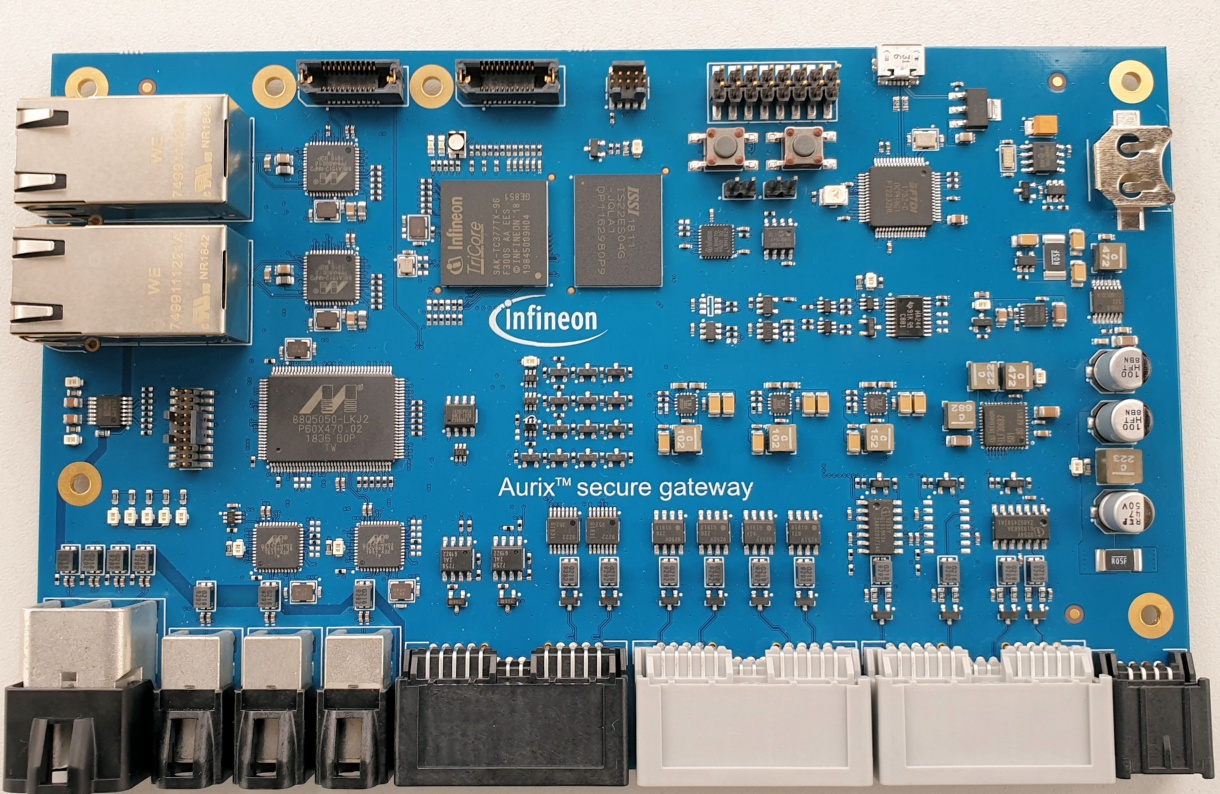
\includegraphics[width=0.8\textwidth]{img/secure-gateway.jpg}
 \caption{KIT\_A2G\_TC377\_SEC\_GTW}
 \label{fig:gw-photo}
\end{figure}

\begin{figure}[!htb]
 \centering
 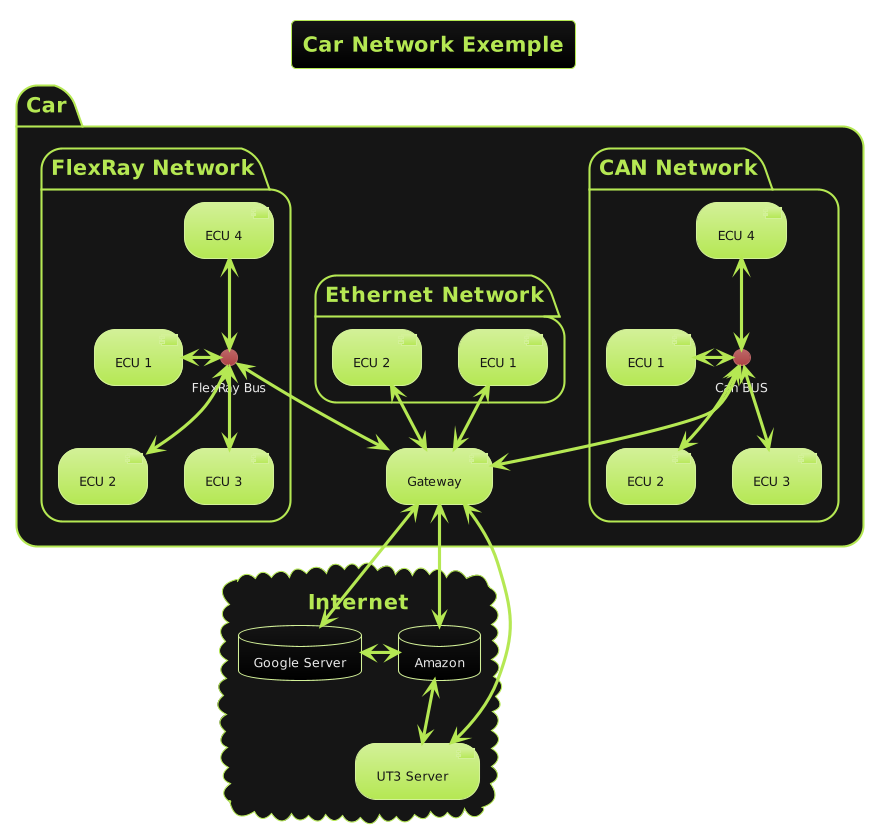
\includegraphics[width=\textwidth]{img/gateway_car.png}
 \caption{Exemple des réseaux interconnect\'ees dans une voiture}
 \label{fig:gw-car}
\end{figure}

\begin{figure}[!htb]
 \centering
 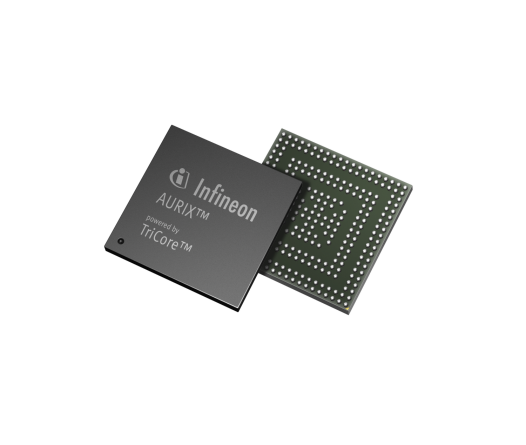
\includegraphics[width=0.5\textwidth]{img/Aurix.png}
 \caption{AURIX (Automotive Realtime Integrated NeXt Generation Architecture)}
 \label{fig:aurix-photo}
\end{figure}

Le syst\`eme d'exploitation est fournie avec une petite demo technique qui sert pour la prise en main de la gateway et tester son fonctionnement basique de connecter 2 reseaux avec des protocoles physiques et logiques incompatibles. Pour lancer la demo il est necessaire de connecter 2 ECU externes \`a certains ports CAN et Ethernet du gateway, voir figures \ref{fig:gw-demo-uc1} et \ref{fig:gw-demo-uc2} pour plus d'information concernant aux connections. La demo a 2 cas d'utilisation :

%El gateway viene con un programa de demostracion que pretende hacer la prise en main del gateway, testear el funcionamiento basico y mostrar las capacidades del mismo. Para testear el Demo es necesario conectar 2 ECU's externar a ciertos puertos especificados en la figura \ref{fig:connections-diagram}. El demo en cuestion tiene 2 use Cases los cuales vamos a explicar por separado.

\begin{itemize}
    \item Use Case 1 : L'ECU connect\'e au port CAN envoie une trame d'information qui sera reenvoy\'e vers l'ECU en Ethernet (fig. \ref{fig:gw-demo-uc1}).%En este Use Case se envia un frame can y el gateway le hace forward por puerto ethernet. Retratado en la figura \ref{fig:gw-demo-uc1}.
    \item Use Case 2 : L'ECU connect\'e au port Ethernet envoie une trame d'information qui sera reenvoy\'e vers l'ECU en CAN (fig. \ref{fig:gw-demo-uc2}).%En Este Use case se envia un frame ethernet y esto se le hace forward hacia un bus can. Retratado en la figura \ref{fig:gw-demo-uc2}.
\end{itemize}

\begin{figure}[!htb]
 \centering
 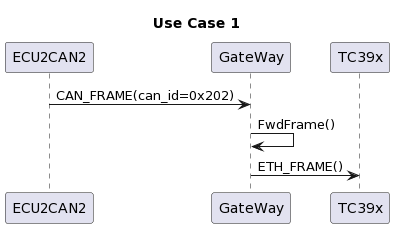
\includegraphics[width=0.7\textwidth]{img/GWUseCase1.png}
 \caption{Gateway Demo Use Case 1}
 \label{fig:gw-demo-uc1}
\end{figure}

\begin{figure}[!htb]
 \centering
 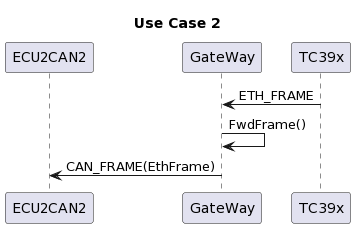
\includegraphics[width=0.7\textwidth]{img/GWUseCase2.png}
 \caption{Gateway Demo Use Case 2}
 \label{fig:gw-demo-uc2}
\end{figure}

Pour tester le fonctionnement basique de cette gateway il nous faut toute une infrastructure comme une reseaux CAN, des ECU compatibles, un banc de tests, outils de vérification, etc, ce nous présente les probl\`emes suivants:
\begin{itemize}
    \item - Construction d'une espace contr\^ol\'e et securis\'e pour accueillir ces composants.
    \item - Haute coûte d'achats des composants pour tester qui pourront ne pas être disponibles vu la situation actuelle des semiconducteurs.
    \item - Fabrication des bancs de test.
    \item - Frais des maintenance future pour maintenir le bon fonctionnement du banc de test.  
\end{itemize}

Toute ces probl\`emes augmentent le co\^ut et la dur\'ee du projet, et si les besoins du projet changent il sera nécessaire changer des composants ou fabriquer des nouvelles pièces de hardware. Dans une cadre du développement de logiciel ce n'est pas le cas le plus efficace.

\subsection{Objectifs du projet}

ASTC Design Partners veut virtualiser cette gateway en utilisant son outil VLAB Works. Avec une solution virtualis\'e non seulement les coûts de fabrication, délais de livraison et maintenance seront evit\'es mais aussi le développement de tests automatis\'es sera plus rapide, chaque développeur aura son propre banc de test personalis\'es et les bugs software seront trouves plus facilement. 

%La propuesta de ASTC Desing Partners es virtualizar este Gateway para poder agilizar el proceso del desarrollo de software, sobretodo en un contexto de escasez mundial de microcontroladores. Ademas, es bien sabido que suele haber pocas unidades disponibles para testear por lo que es mejor tenerlo digitalizado para que cada programador pueda avanzar por su lado sin necesidad de hacer cola por el hardware, a menos que sea necesario.

Au début du projet nous avions disponible VLAB, le mod\`ele virtualis\'e du microcontr\^oleur \textit{AURIX TC37x} utilis\'e dans la gateway et le software compil\'e MICROSAR fournie avec la gateway. Le software de la gateway doit verifier le fonctionement correct de toutes les componsants et buses de donn\'ees presents sur la gateway. A fin de virtualiser la gateway, il faut remplir quelques objectifs basiques : 
\begin{itemize}
    \item - Modéliser des composants nécessaires pour que le syst\`eme d'exploitation démarre.
    \item - Faire un testbench avec les bus de donn\'ees necessaires pour l'envoie des donn\'ees.
    \item - Augmenter les capacit\'es du \textit{TC37x} parce que la gateway utilise une version amelior\'e de ce microcontr\^oleur appell\'e par infineon \textit{TC37xEXT}\cite{aurix.tc37e}.
\end{itemize}